\documentclass{svproc}
\usepackage{url}
\def\UrlFont{\rmfamily}
\usepackage{graphicx}
\usepackage{amsmath}

\emergencystretch=3em
\begin{document}
\mainmatter
\title{Online Modelling for Real-Time Chiller Efficiency Optimization: A Verified Co-Simulation Testbed with Load Forecasting, Online Efficiency Tracking and Staging-Decision Analysis}
\titlerunning{Online Modelling for Chiller Efficiency Optimization}
\author{Mohammad Esmail \and Tong Yuen Chai}
\authorrunning{M.\ Esmail and T.\ Y.\ Chai}
\institute{Universiti Tunku Abdul Rahman (UTAR), Malaysia\\
\email{moh.esmail@gmail.com, chaity@utar.edu.my}}
\maketitle

\begin{abstract}
Chiller plants account for a large share of commercial-building electricity, yet most run on fixed sequencing rules tuned at commissioning. We describe a reproducible co-simulation testbed (3R2C building, three-chiller water-cooled plant with DOE-2 ``Electric EIR'' curves, time-of-use tariff) with a verified conventional baseline, and add a learning layer to it: a walk-forward-evaluated gradient-boosting load forecaster, and recursive-least-squares (RLS) estimators that track efficiency drift online. A quasi-static decision analysis then asks how much each kind of model error matters for the discrete choice of how many chillers to run. On synthetic data, forecasting reaches CV(RMSE) of 2.1\,\%, 3.2\,\% and 5.3\,\% at 15\,min, 1\,h and 4\,h; online RLS halves one-step power-prediction error under injected drift (2.8\,\% vs.\ 5.5\,\%). Staging analysis gives a more sober message: errors in model \emph{scale} (efficiency level $\pm30\,\%$) and realistic forecast errors change the stage-count decision by well under 0.1\,\% of plant energy, whereas errors in the part-load curve \emph{shape} cost up to 2.8\,\%, and the rule-based sequencer itself leaves 1.4--3.3\,\% on the table. All results come from simulation with placeholder tariffs; code is provided for exact reproduction.
\keywords{chiller plant, online identification, recursive least squares, load forecasting, model predictive control, co-simulation}
\end{abstract}

\section{Introduction}
Heating, ventilation and air-conditioning (HVAC) is among the largest electrical end uses in commercial buildings, and in tropical climates the chilled-water plant dominates it. Chiller performance is not static: condenser fouling, refrigerant charge, wear and changing load patterns move the efficiency surface away from its commissioning state, while staging decisions---how many chillers to run---are still commonly made by threshold rules. Model predictive control (MPC) with forecasts is the natural remedy \cite{afram2014,oldewurtel2012,sturzenegger2016}, but its benefit depends on two things that are rarely quantified together: how well the load and the plant efficiency can be predicted, and how much an error in either actually changes the operating decision.

This paper takes a deliberately measurement-first approach. Before any predictive controller is built, we (i) construct a testbed whose numerical correctness and conventional baseline are verified, (ii) add the learning components that MPC would rely on---a load forecaster and an online efficiency tracker---and (iii) quantify, by decision analysis, how their errors propagate into the staging decision. The aim is to establish \emph{where} a learning layer can pay off before committing to a controller. Our contributions are:
\begin{enumerate}
\item an open, verified Python co-simulation testbed with energy-balance, integrator, time-step and rating-standard checks, and a sensitivity analysis showing that the strategy comparison is more robust than absolute consumption (Section~\ref{sec:testbed});
\item a walk-forward evaluation of short-horizon cooling-load forecasting, including the value of an (imperfect) weather forecast (Section~\ref{sec:forecast});
\item a gray-box RLS estimator of chiller efficiency, in scalar and three-parameter forms, evaluated under two injected drift scenarios (Section~\ref{sec:online});
\item a decision analysis separating errors in efficiency \emph{scale}, in part-load \emph{shape} and in load forecasts, with the finding that the first matters little and the second a great deal (Section~\ref{sec:decision}).
\end{enumerate}
\paragraph{Relation to the wider research programme.} This paper reports one part of a larger programme on online modelling and predictive control of chiller plants, whose end goal is a closed-loop MPC with verified efficiency gains. What is reported here is the enabling layer (testbed, forecasting, online identification, decision analysis); the controller itself, its ablation against a static efficiency model, and any claim of achieved savings are \emph{not} part of this paper. The 1.43\,\% figure below is the headroom of better staging on a simulated plant, not a demonstrated saving.

We state limits plainly: all data are simulated, the tariff is a placeholder, the decision analysis is quasi-static, and no closed-loop MPC is reported here (Section~\ref{sec:limits}).

\section{Related Work}
\emph{Chiller modelling.} Regression-based models of the DOE-2 type express electrical input as the product of a rated value and curves in load fraction and temperatures; they are standard in EnergyPlus \cite{crawley2001} and have been studied for calibration from plant data \cite{hydeman2002a,hydeman2002b}. Ratings follow AHRI~550/590 \cite{ahri550}. \emph{Chiller-plant optimisation} has used simplified adaptive models with evolutionary search \cite{ma2011}, quadratic plant representations \cite{ahn2001} and practical sequencing guidance \cite{hydeman2007}. \emph{Predictive control} of buildings with weather forecasts is reviewed in \cite{afram2014}; field trials report cost benefit \cite{sturzenegger2016}, and learning-based control is surveyed in \cite{wang2020}. \emph{Load prediction.} Data-driven building energy prediction is reviewed in \cite{amasyali2018}; gradient-boosted trees \cite{friedman2001} remain highly competitive on tabular inputs \cite{grinsztajn2022}, and time-series evaluation needs forward-chaining rather than random splits \cite{bergmeir2012}. \emph{Online identification.} RLS with forgetting is a classical tool for tracking slowly varying parameters \cite{ljung1999,astrom1995,haykin2002}; gray-box building models are discussed in \cite{braun2002,bacher2011}. To our knowledge, what is less often reported is the separation we make here between error in efficiency level, in part-load shape, and in load forecast, each measured in units of staging-decision loss. This statement about the literature has not yet been established by a systematic review and should be read as a hypothesis motivating the study.

\section{Testbed and Baseline}\label{sec:testbed}
\subsection{Architecture}
Weather, building, plant, tariff and controller are separate modules with fixed interfaces, coupled at a 15-minute step (Fig.~\ref{fig:arch}). The controller is the only block that changes between conventional control and the learning-based variants.

\begin{figure}[t]
\centering
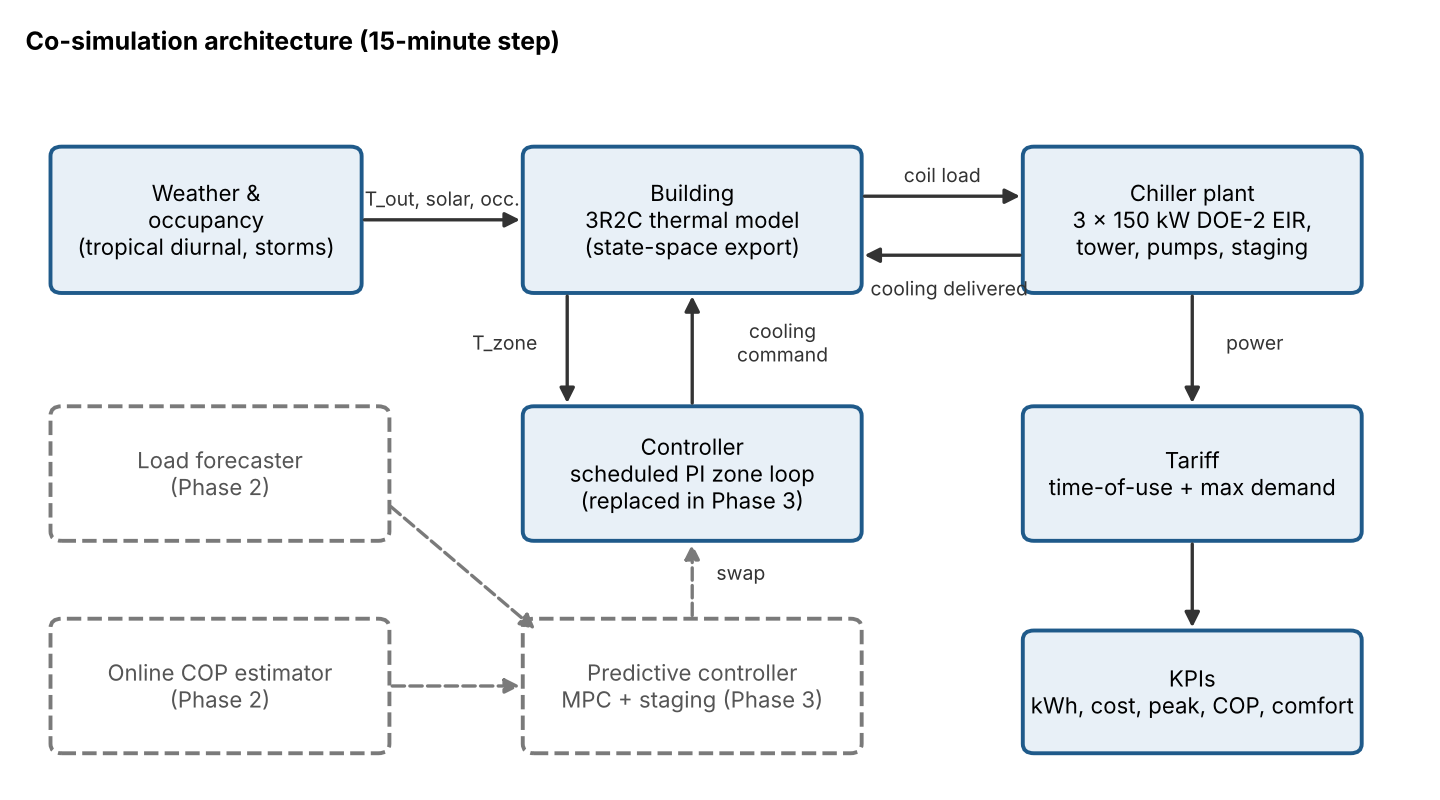
\includegraphics[width=\textwidth]{figs/fig1_architecture.png}
\caption{Co-simulation architecture. Solid blocks are implemented; the learning layer (Sections~\ref{sec:forecast}--\ref{sec:online}) attaches to the same interfaces.}
\label{fig:arch}
\end{figure}

\paragraph{Building.} A 3R2C lumped thermal model of a $\approx 5{,}000\,\mathrm{m^2}$ office (two thermal modes, time constants 0.85\,h and 10.4\,h), driven by a synthetic tropical weather generator with cloud variability and afternoon storms. The model exports its continuous-time state-space matrices, so a predictive controller can use the same dynamics without reformulation. Latent load is a fixed multiplier (1.3) on sensible load. Peak coil load is about 361\,kW.

\paragraph{Plant.} Three 150\,kW constant-speed water-cooled centrifugal chillers use the DOE-2 form
\begin{equation}
\begin{split}P_{ch} &= n\,\frac{C(T_{cw})}{\mathrm{COP}_{ref}}\;\mathrm{EIRfT}(T_{chw},T_{cw})\;\mathrm{EIRfPLR}(\mathrm{PLR}),\\ \mathrm{EIRfPLR}&=a+b\,\mathrm{PLR}+c\,\mathrm{PLR}^2,\end{split}
\label{eq:chiller}
\end{equation}
with $n$ running units sharing the load, $a+b+c=1$ (nominal $a,b,c=0.30,0.23,0.47$), and on/off cycling below 15\,\% part-load. A cooling tower (approach 3--5\,K over wet-bulb), variable-speed chilled-water pump, per-unit condenser pumps and tower fans complete the plant. Curve coefficients are \emph{synthetic}, not manufacturer data.

\paragraph{Conventional control.} The baseline is a scheduled plant with a tuned PI zone loop with anti-windup, threshold chiller sequencing (stage up above 90\,\% of unit capacity, down below 75\,\% of the reduced stage) and a fixed supply temperature---deliberately competent, since savings are only meaningful against a credible reference. A second reference, fixed-schedule pre-cooling, is included as an intermediate benchmark.

\subsection{Verification and Baseline Results}
\textbf{Verification} (does the code solve the equations correctly?): against the closed-form matrix-exponential solution of the linear thermal model the RK4 integrator deviates by at most $7.9\times10^{-5}$\,K over 24\,h; first-law closure over 14 days leaves $2.1\times10^{-5}\,\%$ of throughput; and the 15-minute step lies within 0.18\,\% in energy and 0.03\,\% in peak of a 5-minute solution (a 60-minute step would overstate energy by 4.6\,\% and understate peak by 5.1\,\%). \textbf{Plausibility} (not validation): the plant rates at 0.597\,kW/ton full-load and 0.556\,kW/ton IPLV under AHRI~550/590 conditions, and five plant-level metrics (seasonal COP 4.93, peak cooling density 72\,W/m$^2$, auxiliary share 17.7\,\%, tower approach 3.9\,K, daily plant electricity) fall inside indicative ranges. \textbf{Empirical validation against measured plant data has not been done}; the ASHRAE Guideline~14 statistics \cite{ashrae14} (NMBE, CV(RMSE)) are implemented but unrun for lack of data.

Table~\ref{tab:base} gives 14-day results (two spin-up days discarded). Rule-based pre-cooling is \emph{worse} than the baseline on cost by 7.3\,\%: it saves RM\,23 of energy charge but creates a new 04:30 demand peak (90.4 vs.\ 72.2\,kW) and uses 4.2\,\% more energy. This negative result separates ``prediction helps'' from the weaker ``any load shifting helps''. Under $\pm25\,\%$ perturbation of eight building parameters, absolute energy moved by $-25$ to $+26\,\%$ (the model is uncalibrated), but the energy gap between the two strategies stayed within 3.8--5.9\,\% (nominal 4.2\,\%) in all 16 cases, because parameter error is largely common to both strategies. The cost gap (0--12.4\,\%) is less robust because the demand charge hinges on a single interval; costs here use placeholder RM rates and indicate direction only.

\begin{table}[t]
\caption{Baseline and rule-based pre-cooling, 14 simulated days (placeholder tariff).}
\label{tab:base}
\centering
\begin{tabular}{lrrrr}
\hline\noalign{\smallskip}
Strategy & Energy (kWh) & Cost (RM) & Peak (kW) & Plant COP \\
\noalign{\smallskip}\hline\noalign{\smallskip}
Schedule + PI & 7,665 & 3,203 & 72.2 & 4.93 \\
Pre-cooling & 7,987 & 3,437 & 90.4 & 4.97 \\
\noalign{\smallskip}\hline
\end{tabular}
\end{table}

\subsection{Non-Convex Efficiency Surface}
Mapping plant COP over load and wet-bulb temperature (Fig.~\ref{fig:cop}) shows that efficiency rises to a local peak just below each stage-up threshold and then drops as the next unit starts: by 12\,\% at the first threshold (COP 5.13 to 4.51 at 25\,\textdegree C wet-bulb) and 3\,\% at the second. The surface depends weakly on wet-bulb compared with load. The drops depend on the assumed part-load curve and auxiliary power and are therefore properties of this synthetic plant. The surface implies a discrete decision that a continuous model cannot represent---which motivates Section~\ref{sec:decision}.

\begin{figure}[t]
\centering
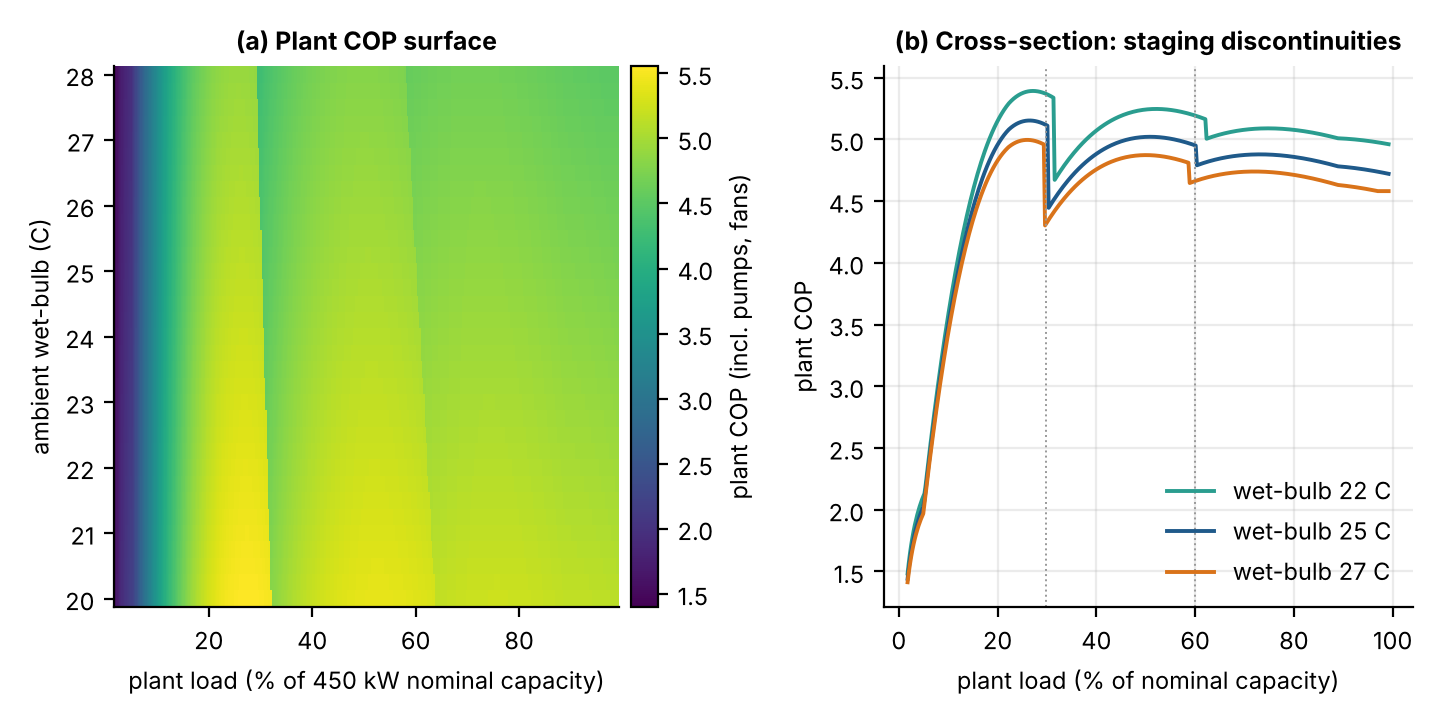
\includegraphics[width=\textwidth]{figs/fig4_cop_surface.png}
\caption{Plant COP over the operating envelope; staging produces sharp discontinuities.}
\label{fig:cop}
\end{figure}

\section{Cooling-Load Forecasting}\label{sec:forecast}
\paragraph{Setup.} The testbed was run for 120 days under the baseline strategy; the forecasting target is the coil load $H$ steps ahead ($H\in\{1,4,16\}$, i.e.\ 15\,min, 1\,h, 4\,h), evaluated during scheduled hours (06:00--18:30), about 4{,}600 points per horizon. Inputs are time of day (sine/cosine), occupancy, current and lagged loads ($t$, $t{-}15$, $t{-}30$, $t{-}60$\,min), zone temperature, current weather, the load at the same time the previous day, and a \emph{noisy weather forecast} for the target time (dry-bulb, solar and humidity with error standard deviations that grow with horizon: 0.3/0.6/1.2\,K, 5/10/25\,\% and 1.5/3/6\,\% RH). Models: persistence, seasonal-naive (yesterday), ridge regression and histogram gradient boosting (HGB, scikit-learn \cite{pedregosa2011}). Evaluation is \emph{walk-forward}: initial training on 28 days, then 14 successive 7-day test folds with an expanding training window, never training on the future. Accuracy is CV(RMSE)$=100\sqrt{\overline{e^2}}/\bar y$. Errors $e$ are pooled over all test points (no degrees-of-freedom correction), and $\bar y$ is the mean observed coil load over the same points ($\approx 244$\,kW, scheduled hours only); the figure is therefore not identical to the hourly CV(RMSE) of Guideline~14 \cite{ashrae14}, which is defined for calibration, not forecasting. The metric was recomputed independently of the reporting code, and the training window of every fold ends before the first test target.

\begin{table}[t]
\caption{Walk-forward load-forecast accuracy, CV(RMSE) in \%, noisy weather forecast.}
\label{tab:forecast}
\centering
\begin{tabular}{lrrr}
\hline\noalign{\smallskip}
Model & 15 min & 1 h & 4 h \\
\noalign{\smallskip}\hline\noalign{\smallskip}
Persistence & 20.4 & 30.5 & 51.6 \\
Seasonal naive & 10.0 & 10.0 & 10.0 \\
Ridge & 3.2 & 6.6 & 8.2 \\
Gradient boosting (HGB) & \textbf{2.1} & \textbf{3.2} & \textbf{5.3} \\
\noalign{\smallskip}\hline
\end{tabular}
\end{table}

\paragraph{Results.} Table~\ref{tab:forecast} and Fig.~\ref{fig:fcst} show HGB beating every baseline at every horizon, with a skill of about 0.90 over persistence in RMSE; errors rise with horizon but stay within 5.3\,\% at 4\,h and are stable across folds (4\,h: 3.4--6.7\,\%). A weather forecast helps mainly at longer horizons: at 4\,h CV(RMSE) is 4.0\,\% with a perfect forecast, 5.3\,\% with the noisy one and 5.8\,\% without; at 15\,min it is irrelevant (2.1--2.2\,\%). Because the load here is generated by a smooth deterministic model plus synthetic weather, these numbers are \emph{optimistic} compared to a real building with irregular occupancy; they show that the pipeline works and how weather-forecast quality enters, not what accuracy to expect on site. A recurrent network was not trained as a comparison.

\begin{figure}[t]
\centering
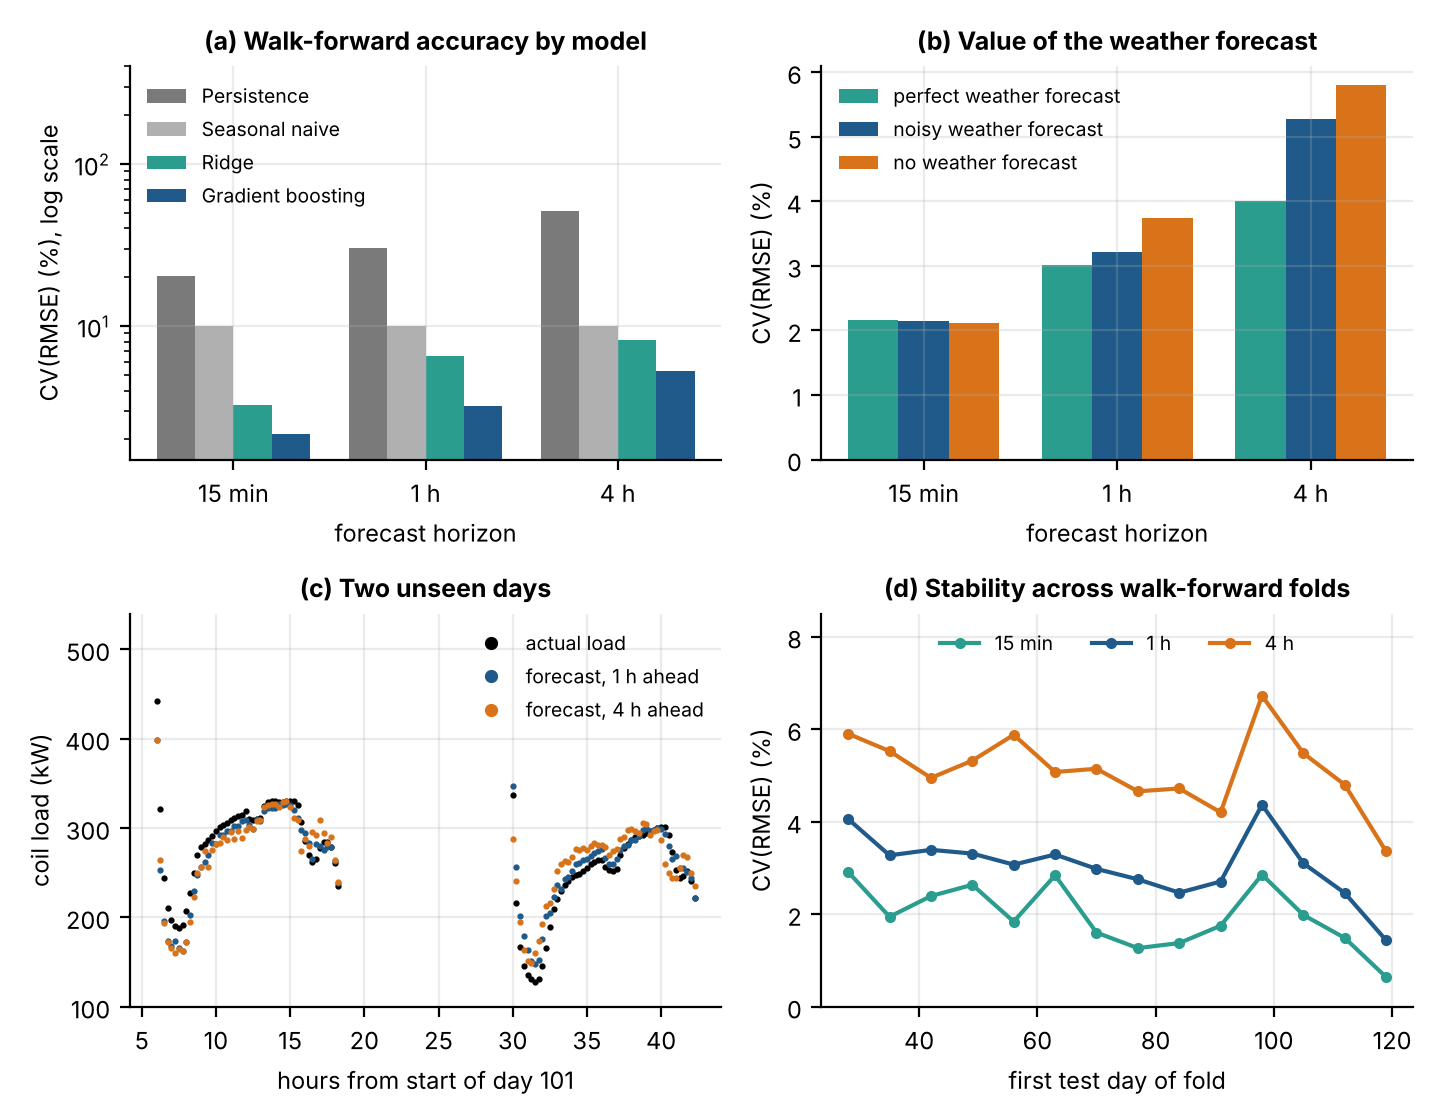
\includegraphics[width=\textwidth]{figs/fig6_forecasting.png}
\caption{Forecasting. (a) accuracy by model and horizon; (b) value of the weather forecast; (c) two unseen days; (d) CV(RMSE) per walk-forward fold.}
\label{fig:fcst}
\end{figure}

\section{Online Efficiency Tracking}\label{sec:online}
\paragraph{Gray-box estimators.} Measured chiller electrical power is modelled on the commissioning structure (\ref{eq:chiller}) with a slowly varying multiplier $k$ (relative COP$^{-1}$): $y_t=k\,\phi_t$, where $\phi_t$ is the commissioning-model power at the observed load, stage count and condenser water temperature, and $y_t$ is sub-metered power with 2\,\% multiplicative noise. The recursive update with forgetting factor $\lambda$ is
\begin{equation}
K_t=\frac{P_{t-1}\phi_t}{\lambda+\phi_t^2P_{t-1}},\quad \hat k_t=\hat k_{t-1}+K_t(y_t-\hat k_{t-1}\phi_t),\quad P_t=\frac{P_{t-1}-K_t\phi_tP_{t-1}}{\lambda}.
\end{equation}
Because (\ref{eq:chiller}) is linear in $(a,b,c)$, a three-parameter estimator with vector regressor $\boldsymbol\phi_t=\frac{nC}{\mathrm{COP}_{ref}}\mathrm{EIRfT}\,[1,\mathrm{PLR},\mathrm{PLR}^2]$ follows the same recursion in vector form; samples in the cycling region (PLR\,$<0.15$) are excluded.

\paragraph{Drift scenarios (injected).} (A) \emph{Fouling and cleaning}: efficiency degrades linearly by 10\,\% from day 15 to 60, is restored to $-1\,\%$ by a cleaning at day 60, then degrades 6\,\% over 45 days. (B) \emph{Part-load flattening}: the fixed-loss term $a$ rises from 0.30 to 0.42 over days 20--80 ($b,c$ rescaled so the curve equals 1 at full load). A no-drift control run checks that the estimator does not invent drift (mean $|\hat k-1|=0.05\,\%$).

\paragraph{Results.} The metric is the one-step-ahead power prediction error (before the update) against the static commissioning model, which has error 5.45\,\% in scenario~A (7--9\,\% at the end of fouling episodes; Fig.~\ref{fig:online}b). With $\lambda=0.998$ the RLS error is 2.76\,\% (mean parameter error 1.3\,\%); with $\lambda=0.99$ it is 2.26\,\% (0.44\,\%); with $\lambda=1$ (no forgetting) 3.38\,\% (2.2\,\%), since it cannot follow the cleaning event. Meter noise of 2\,\% sets a floor, and the parameter error is nearly insensitive to noise up to 5\,\% (Fig.~\ref{fig:online}d). Shorter memory tracks faster at the cost of noise sensitivity (0.43\,\% $\to$ 0.53\,\% mean error as noise rises 0.5\,\% $\to$ 5\,\% at $\lambda=0.99$), which is the expected bias--variance trade-off. In scenario~B the scalar $k$ cannot represent a change of \emph{shape}: its error is 3.41\,\%, against 2.57\,\% for the three-parameter curve and 6.50\,\% for the static model. The curve estimator lags the true parameter (Fig.~\ref{fig:online}c): the regressors $[1,\mathrm{PLR},\mathrm{PLR}^2]$ are collinear over the operating range, so individual coefficients are weakly identifiable even when predictions are accurate. We therefore report prediction error, and warn that estimated coefficients should not be read as physical quantities.

\begin{figure}[t]
\centering
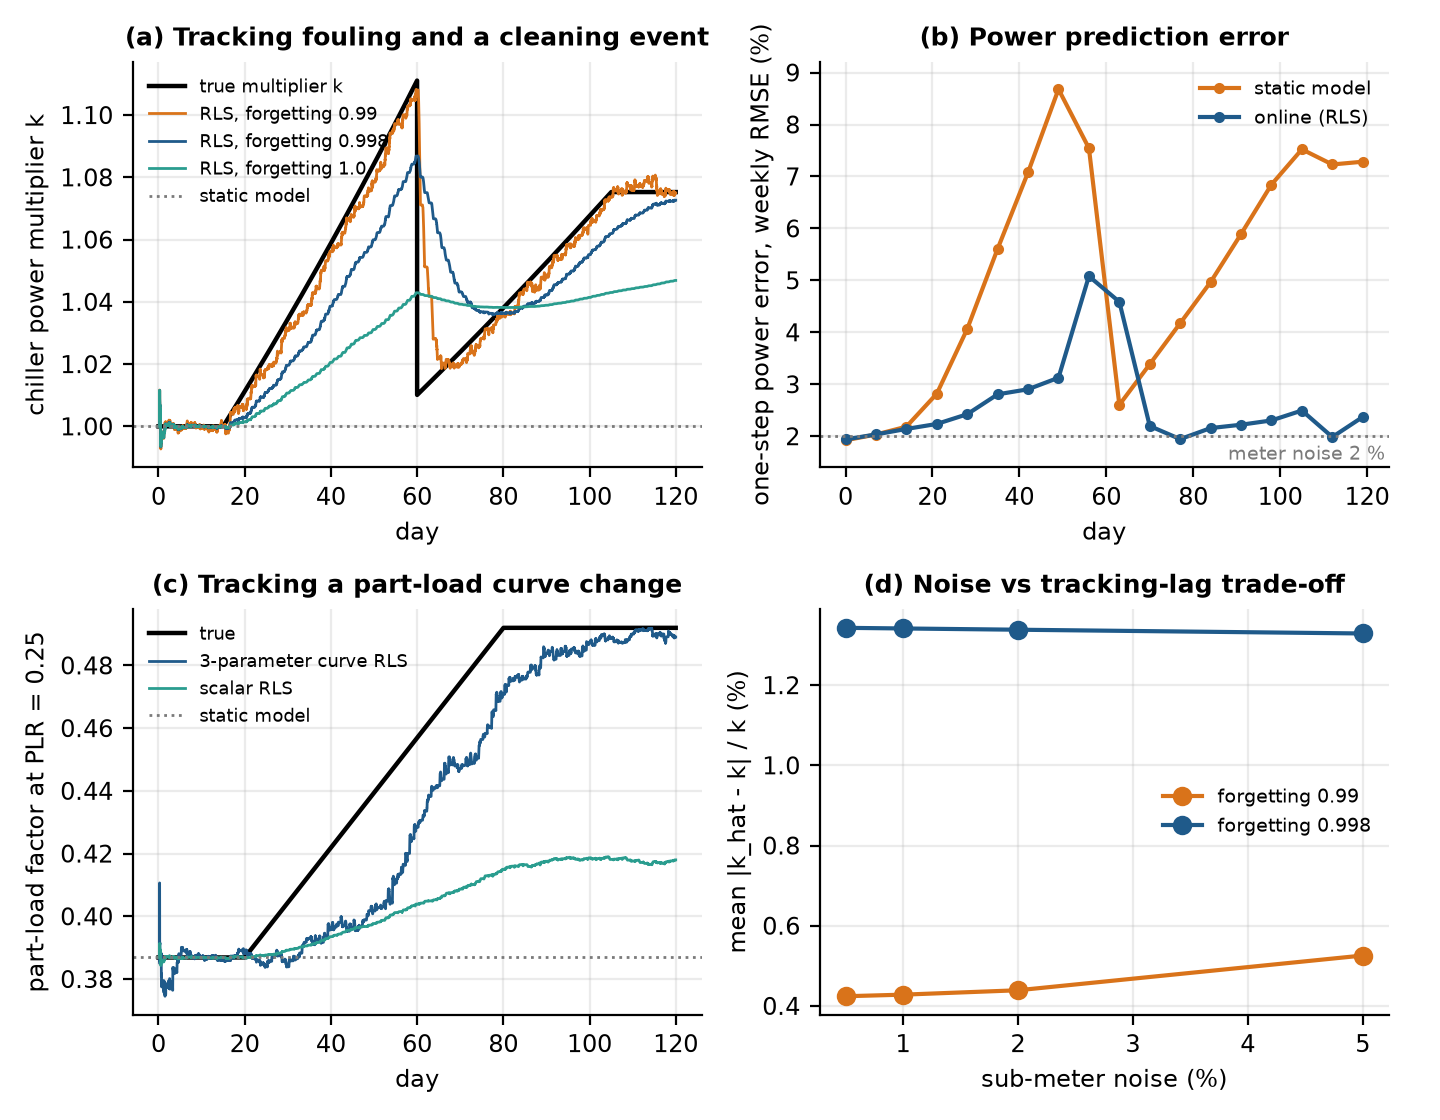
\includegraphics[width=\textwidth]{figs/fig7_online_identification.png}
\caption{Online identification. (a) tracking of the multiplier $k$ through fouling and cleaning; (b) weekly power-prediction error; (c) tracking of the part-load factor at PLR\,$=0.25$; (d) noise versus forgetting.}
\label{fig:online}
\end{figure}

\section{How Much Do Model and Forecast Errors Matter for Staging?}\label{sec:decision}
\paragraph{Method.} At each scheduled time step with load $q$ and wet-bulb temperature $T_{wb}$, the quasi-static plant electrical power (chillers, pumps, fans) is evaluated for each feasible stage count $n\in\{1,2,3\}$; the \emph{optimal} $n^\ast$ minimises it under the \emph{true} plant. A decision-maker with an imperfect model (or forecast) picks $\hat n$ from its own estimate; we report the \emph{mismatch rate} ($\hat n\neq n^\ast$) and the \emph{excess energy} $\sum P(\hat n)/\sum P(n^\ast)-1$ evaluated on the true plant. This is a measure of \emph{decision regret}, not of closed-loop savings: it ignores dynamics, ramp constraints and the thermal-storage value of the building, which is where predictive control would add more.

\paragraph{Headroom.} Over 6{,}000 scheduled steps, the rule-based sequencer chooses a different stage count from the quasi-static optimum on 35.9\,\% of steps and uses 1.43\,\% more plant energy (74.4 vs.\ 73.3\,MWh over the run). This is an \emph{upper bound on what better staging alone can recover} on this plant, before any thermal-storage value; the mismatch concentrates in the 20--40\,\% and 55--70\,\% load bands (Fig.~\ref{fig:dec}d).

\paragraph{Errors in scale do not matter.} Giving the decision-maker a model with the efficiency level wrong by factors of 0.8--1.3 changes the plant energy by at most 0.010\,\% (mismatch 1--3\,\%). Likewise under fouling drift (scenario~A) a static model loses only $2.6\times10^{-4}\,\%$ and online RLS $3\times10^{-5}\,\%$ versus 1.42\,\% for the rule-based sequencer. The reason is structural: the chiller multiplier $k$ scales every candidate stage count almost equally, so the ranking of options is unchanged. \emph{Consequently, online tracking of efficiency \emph{level} is valuable for diagnostics, prediction and MPC cost forecasting, but not for choosing the stage count on this plant.} This corrects an expectation we held at the outset---that small model errors flip the staging choice near thresholds.

\paragraph{Errors in shape matter.} Errors in the part-load curve parameter $a$ do: with $a=0.15$ the extra energy is 2.83\,\% (mismatch 58\,\%) and with $a=0.22$ it is 0.98\,\% (33\,\%), whereas for $a\ge0.38$ the results are identical (1.9\,\% mismatch, 0.005\,\%), consistent with the choice saturating at the minimum feasible number of units. Under part-load drift (scenario~B) the static model loses 0.10\,\%, the scalar RLS 0.13\,\% (slightly \emph{worse}: a scalar absorbs shape error in the wrong direction), the three-parameter curve RLS $0.001\,\%$, and the rule-based sequencer 3.32\,\%. Identification therefore pays off for staging only if the estimator can represent the kind of drift that occurs.

\paragraph{Forecast errors.} Replacing the true load by a forecast $\hat q=q(1+\sigma\varepsilon)$ with random relative error $\sigma$ yields excess energy 0.11, 0.29, 0.66, 0.98 and 1.19\,\% at $\sigma=5,10,20,30,40\,\%$ (mismatch 6--23\,\%), i.e.\ roughly linear in $\sigma$ and always below the 1.43\,\% rule-based loss (Fig.~\ref{fig:dec}a). Using the actual HGB forecasts of Section~\ref{sec:forecast}, the staging loss is 0.031, 0.060 and 0.100\,\% for 15\,min, 1\,h and 4\,h horizons (mismatch 1.6, 3.2, 5.0\,\%). At the accuracy achieved on this synthetic data, forecast error costs one to two orders of magnitude less than the rule-based sequencer's own loss; the accuracy threshold at which a forecast stops being useful for staging is reached only at relative errors well beyond 40\,\%. Real-building forecasts will be worse than ours, and the threshold should be re-estimated on measured data.

\begin{figure}[t]
\centering
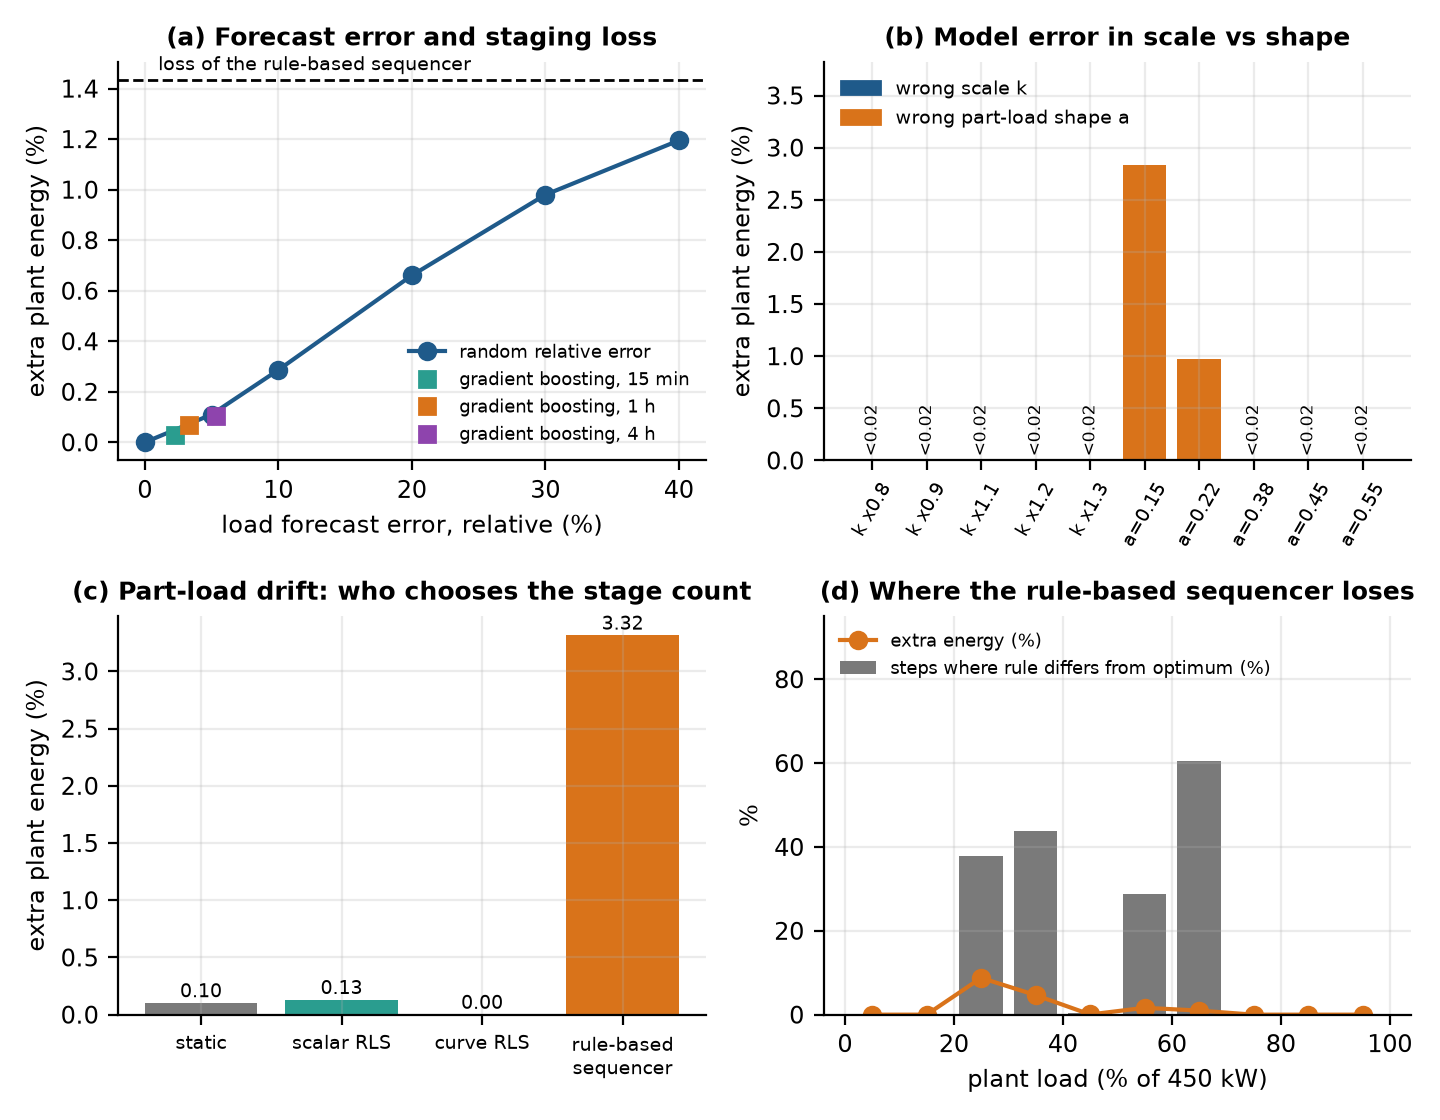
\includegraphics[width=\textwidth]{figs/fig8_staging_decisions.png}
\caption{Decision analysis. (a) staging loss versus load-forecast error (dashed: rule-based sequencer's loss); (b) model error in scale versus shape; (c) who chooses the stage count under part-load drift; (d) where the rule-based sequencer loses, by load band.}
\label{fig:dec}
\end{figure}

\section{Discussion and Limitations}\label{sec:limits}
\paragraph{What the evidence supports.} Within this testbed: (1) load forecasting to a few per cent CV(RMSE) is achievable and leaves staging regret negligible; (2) online RLS substantially improves power prediction under drift and is cheap; (3) for the discrete staging decision, \emph{scale} information is nearly irrelevant, \emph{shape} information matters, and the existing rule is itself the dominant loss (1.4--3.3\,\%). The latter suggests that the main near-term value of a learning layer lies in correcting the sequencing rule and in providing accurate costs to an optimiser, rather than in sharpening an efficiency level.

\paragraph{What it does not support.} (i) \emph{All data are simulated}; drift scenarios are injected and the forecaster, the estimators and the plant share the same structural assumptions (the gray-box estimator uses the exact DOE-2 form that generated the data), so structural model error is not tested. (ii) The tariff rates are placeholders; costs indicate direction only, and the baseline's calibration to a real building is absent (Section~\ref{sec:testbed}). (iii) The decision analysis is quasi-static: it omits ramping, minimum run times, thermal storage and comfort constraints, and no closed-loop MPC or ablation (static versus online model) is reported. (iv) Staging losses of 1.4--3.3\,\% are plant-energy figures from a synthetic constant-speed plant; variable-speed machines flatten the part-load structure and could change the conclusions. (v) No recurrent-network baseline was trained, and a Gaussian-process estimator was not tried.

\paragraph{Next steps.} Replace synthetic data with measured BMS trends (enabling Guideline~14 calibration), close the loop with an enumeration-based MPC over the exported state-space model and run the ablation that isolates the online model, and test variable-speed plants.

\section{Conclusion}
We built and verified a chiller-plant co-simulation testbed, added a forecasting and online-identification layer, and measured how its errors translate into staging-decision loss. On synthetic data, forecasting and RLS are accurate and cheap, but the staging decision is robust to errors in efficiency scale and to realistic forecast errors; it is sensitive to the part-load shape, and the existing rule-based sequencer is the largest identified loss. These results define where a learning layer has the most to offer and where it does not, and they set the experimental frame for a predictive controller.

\paragraph{Reproducibility.} The full code, README and expected outputs (Phase~1 and~2; one script reproduces all 24 reported key numbers in about two minutes; Python~3.13, NumPy, SciPy, scikit-learn, Matplotlib) accompany this paper: \url{https://github.com/mesmail/NLPIR_paper_chiller_efficiency}.

\begin{thebibliography}{99}
\bibitem{afram2014} Afram, A., Janabi-Sharifi, F.: Theory and applications of HVAC control systems -- a review of model predictive control (MPC). Build. Environ. 72, 343--355 (2014)
\bibitem{oldewurtel2012} Oldewurtel, F., et al.: Use of model predictive control and weather forecasts for energy efficient building climate control. Energy Build. 45, 15--27 (2012)
\bibitem{sturzenegger2016} Sturzenegger, D., Gyalistras, D., Morari, M., Smith, R.S.: Model predictive climate control of a Swiss office building: implementation, results, and cost-benefit analysis. IEEE Trans. Control Syst. Technol. 24(1), 1--12 (2016)
\bibitem{crawley2001} Crawley, D.B., et al.: EnergyPlus: creating a new-generation building energy simulation program. Energy Build. 33(4), 319--331 (2001)
\bibitem{hydeman2002a} Hydeman, M., Gillespie, K.L.: Tools and techniques to calibrate electric chiller component models. ASHRAE Trans. 108(1), 733--741 (2002)
\bibitem{hydeman2002b} Hydeman, M., Webb, P., Sreedharan, P., Blanc, S.: Development and testing of a reformulated regression-based electric chiller model. ASHRAE Trans. 108(2), 1118--1127 (2002)
\bibitem{ahri550} AHRI Standard 550/590: Performance rating of water-chilling and heat pump water-heating packages using the vapor compression cycle. Air-Conditioning, Heating, and Refrigeration Institute
\bibitem{ma2011} Ma, Z., Wang, S.: Supervisory and optimal control of central chiller plants using simplified adaptive models and genetic algorithms. Appl. Energy 88(1), 198--211 (2011)
\bibitem{ahn2001} Ahn, B.-C., Mitchell, J.W.: Optimal control development for chilled water plants using a quadratic representation. Energy Build. 33(4), 371--378 (2001)
\bibitem{hydeman2007} Hydeman, M., Zhou, G.: Optimizing chilled water plant control. ASHRAE J. 49(6), 44--54 (2007)
\bibitem{wang2020} Wang, Z., Hong, T.: Reinforcement learning for building controls: the opportunities and challenges. Appl. Energy 269, 115036 (2020)
\bibitem{amasyali2018} Amasyali, K., El-Gohary, N.M.: A review of data-driven building energy consumption prediction studies. Renew. Sustain. Energy Rev. 81, 1192--1205 (2018)
\bibitem{friedman2001} Friedman, J.H.: Greedy function approximation: a gradient boosting machine. Ann. Stat. 29(5), 1189--1232 (2001)
\bibitem{grinsztajn2022} Grinsztajn, L., Oyallon, E., Varoquaux, G.: Why do tree-based models still outperform deep learning on typical tabular data? In: NeurIPS Datasets and Benchmarks Track (2022)
\bibitem{bergmeir2012} Bergmeir, C., Ben\'itez, J.M.: On the use of cross-validation for time series predictor evaluation. Inf. Sci. 191, 192--213 (2012)
\bibitem{ljung1999} Ljung, L.: System Identification: Theory for the User, 2nd edn. Prentice Hall (1999)
\bibitem{astrom1995} {\AA}str\"om, K.J., Wittenmark, B.: Adaptive Control, 2nd edn. Addison-Wesley (1995)
\bibitem{haykin2002} Haykin, S.: Adaptive Filter Theory, 4th edn. Prentice Hall (2002)
\bibitem{braun2002} Braun, J.E., Chaturvedi, N.: An inverse gray-box model for transient building load prediction. HVAC\&R Res. 8(1), 73--99 (2002)
\bibitem{bacher2011} Bacher, P., Madsen, H.: Identifying suitable models for the heat dynamics of buildings. Energy Build. 43(7), 1511--1522 (2011)
\bibitem{pedregosa2011} Pedregosa, F., et al.: Scikit-learn: machine learning in Python. J. Mach. Learn. Res. 12, 2825--2830 (2011)
\bibitem{ashrae14} ASHRAE: Guideline 14-2014: Measurement of Energy, Demand, and Water Savings. ASHRAE, Atlanta (2014)
\end{thebibliography}
\end{document}
